% !TEX root = ../../main.tex


\begin{figure}[p]
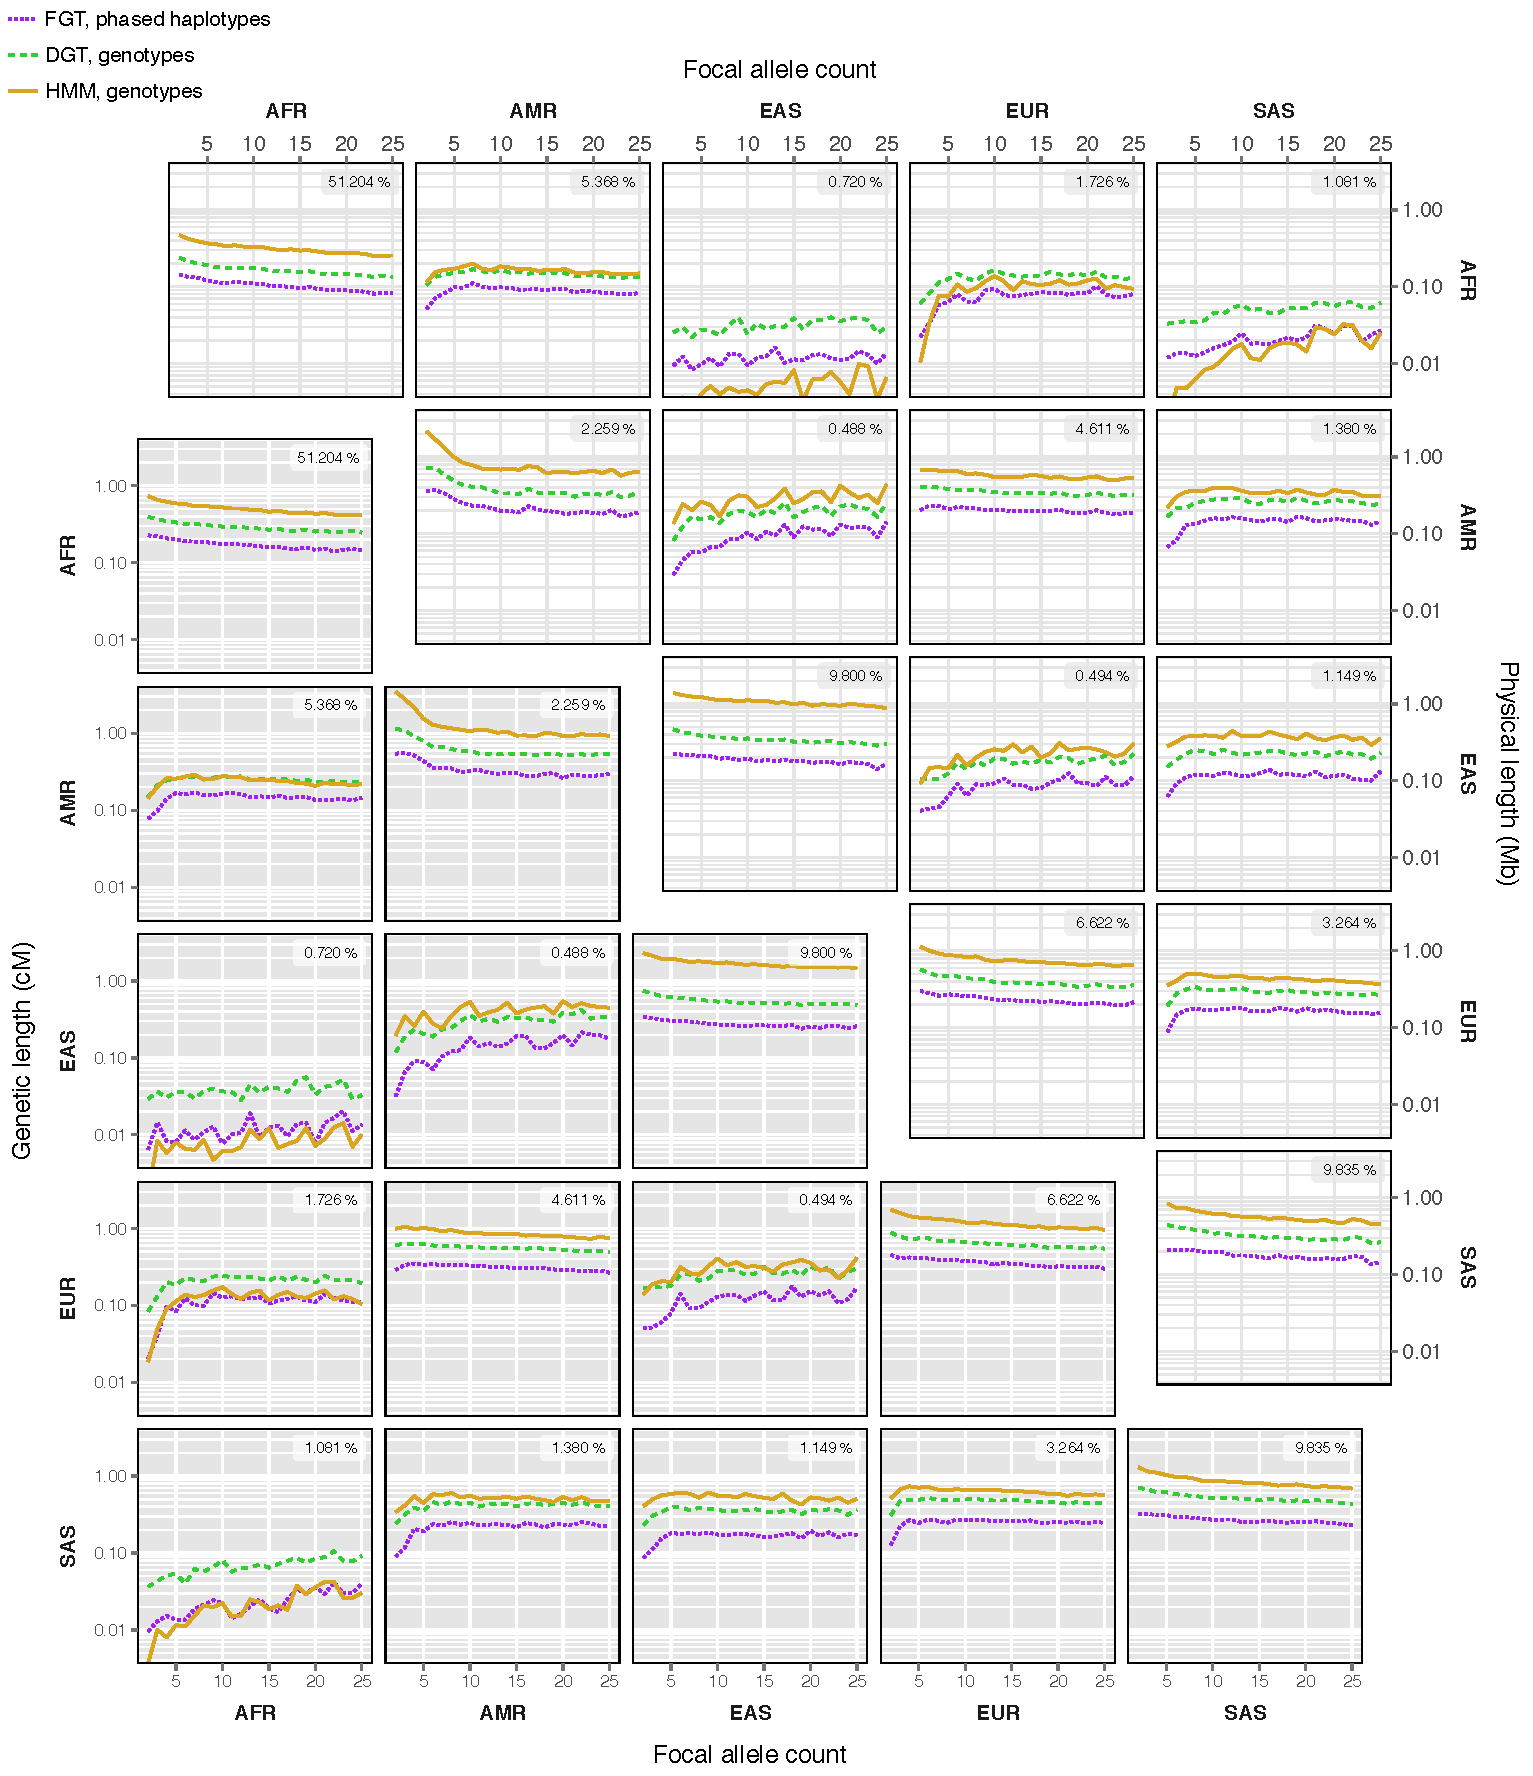
\includegraphics[width=\textwidth]{./img/ch4/1KG_chr20_pop_len}
\Caption{Inferred shared haplotype lengths by population in 1000 Genomes, chromosome 20}
{The distributions of physical (upper triangle) and genetic (lower triangle) length by frequency of the focal allele are shown for alleles shared between pairs of individuals from the same population (\emph{diagonal} panels) and any of the other populations sampled in \gls{1kg}.
Results are shown for shared haplotype lengths inferred using the \gls{fgt}, \gls{dgt}, and \gls{hmm}, on the same subset of 1~million randomly selected pairwise segments inferred at target sites found at \fk{[2,25]} (\ie allele frequency below 0.5\%).
The number of pairs available per comparison is given in each panel (upper right corner).
The dataset comprises samples from \n{5} continental populations (or \emph{super-populations});
African~(AFR), Ad-Mixed American~(AMR), East~Asian~(EAS), European~(EUR), and South~Asian~(SAS).
\AdditionLabel}
{fig:1KG_chr20_pop_len}
\end{figure}
